\sectionmark{Systematik der Mikroorganismen}

\section{Einführung}
\begin{enumerate}
\item Warum ist die ribosomale RNA so gut als Marker für die Untersuchung von Verwandtschaftsverhältnissen geeignet?
	
	Die 16S rRNA ist universell in allen bekannten zellulären Organismen verbreitet
	und erfüllt auch in allen dür die gleich Funktionalität verantwortlich.
	Weiterhin lässt sie sich gut isolieren
	und durch Alignemnts lassen sich die Sequenzen verschiedener Organismen sehr gut vergleichen.
	Durch die geringe gesamte Mutationsrate lassen sich gut entfernte Verwandschaften nachweisen.
	Mit einer Analyse von variablen Bereichen ist auch die Untersuchung von näher verwandten Arten gut möglich.

\item Wie geht man bei der Beschreibung eines neuen Organismus vor?
	
	Detaillierte Beschreibung von:
	\begin{itemize}
		\item Physiologische Eigenschaften (Größe, Gram-färbung, Geißel, Form, etc.)
		\item Temperaturbereich
		\item Habitat
		\item Metabolismus
		\item Genetische Eigenschafte (GC-Gehalt, Proteinfunktionen, Plasmide)
	\end{itemize}

	Weiterhin muss ein Typstamm hinterlegt werden,
	der von anderen Froschern angefordert werden kann.

\end{enumerate}

\newpage
\section{Archaea}
\begin{enumerate}
	\item Vergleichen Sie wichtige molekularbiologische und physiologische Eigenschaften der drei Organismenreiche!
		
		In Tabelle \ref{tab:domaenenuberblick} ist eine Übersich über die Eigenschaften der drei Organismenreiche.	

		\begin{table}[h!]
		\begin{center}
		\begin{tabular}{l l l l} 
		\toprule
		Merkmal		&	Bacteria		&	 Archaea				&	 Eukaraya		\\
		\midrule
		Zellkern 	&	nein			&	 nein					&	 ja		\\
		cccDNA		&	ja				&	 ja					&	 nein (linear)			\\
		Histone		&	nein			&	 ja					&	 ja		\\
		Zellwand		&	Murein		&	 kein Murein		&	 kein Murein		\\
		Membranlipid&	Ester			&	 Ether				&	 Ester		\\
		\midrule
		Ribosomen	&	70S			&	 70S					&	 80S		\\
		Ini-tRNA		&	f-Met			&	 Met					&	 Met		\\
		Introns 		&	nein			&	 nein					&	 ja		\\
		ja				&	Operon		&	 ns					&	 nein		\\
		Cap/poly-A 	&	nein			&	 nein					&	 ja		\\
		Plasmide		&	ja				&	 ja					&	 selten		\\
		RNA-Pol			&	ne (4 UE)	&	 viele (8-12 UE)	&	drei (12-14 UE)	\\
		TK-Faktoren		&	nicht nötig	&	 benötigt			&	benötigt		\\
		Promotoren		&	-10, -35		&	 TATA					&	TATA		\\
		\midrule
		Methanbildung		&	nein			&	 ja					&	nein		\\
		S-Reduktion		&	ja				&	 ja					&	nein		\\
		Nitrifizierung	&	ja				&	 nein					&	nein		\\
		Denitrifizierung		&	ja				&	 ja					&	nein		\\
		N-Fixierung		&	ja				&	 ja					&	nein		\\
		Photosynthese		&	ja				&	 nein					&	nein (Plastiden)	\\
		Lithotrophie	&	ja				&	 ja					&	nein		\\
		Grw. > 80°C		&	ja				&	 ja					&	nein		\\
		\bottomrule
		\end{tabular}
		\label{tab:domaenenuberblick}
		\caption{Übersicht über die Eigenschaften der drei Organismenreiche.}
		\end{center}
		\end{table}

	\item Nennen Sie zwei wichtige Gruppen der Euryarchaeota! Wo würden Sie diese Organismen suchen?
		
		\begin{description}
			\item[Pyrococcus] \hfill \\
				An heißen Standorten.
				(Taq-Polymerase, PCR ?)
			\item[Methanogene Euryarchaeota] \hfill \\
				Die Methanbildenden Euryachaeota, 
				die Gruppen \emph{Methanobacterium}, \emph{Methanococcus} und \emph{Methanosarcina},
				bilden Methan in den Biogas-Anlagen von Klärwerken.
		\end{description}
		Insgesamt lassens ich die Euryarchaeota als eine Gruppe von Extremophilen beschreiben.

	\item Wiederholen Sie kurz die wichtigsten Schritte der Methanbildung! Welche Rolle spielen ungewöhnliche Koenzyme bei diesem Stoffwechselweg?

		Siehe Anaerobe Atmung?!
	
	\item Wie schützt Thermoplasma seine Membran vor der hohen Temperatur?

		Thermoplasma besitzt keine Zellwand sondern eine einzigartige Zellmembran.
		Diese besteht aus Tetraether-Lipiden mit Glukose- und Mannoseeinheiten.

	\item Bei der PCR werden DNA-Fragmente zunächst bei 96\textdegree C aufgeschmolzen. Einige Archaea leben bei wesentlich höheren Temperaturen. Daher gibt es zwei Möglichkeiten für deren DNA:
	\begin{enumerate}
		\item Sie haben einzelsträngige DNA. Wie könnte in diesem Fall die Replikation ablaufen?
				
			Die DNA könnte von einer modifizierten RNA-Polymerase abgelesen werden.

		\item Sie haben doppelsträngige DNA. Wie kann der Doppelstrang bei so hohen Temperaturen stabil sein? Entscheiden Sie sich für eine der Möglichkeiten und beantworten Sie die Zusatzfrage!
			
			Die DNA könnte stark verpackt sein und durch einen hohen GC-Gehalt an die hohhen Temperaturen angepasst sein.

	\end{enumerate}
\end{enumerate}
	
\newpage
\section{Bakterien}
\begin{enumerate}
	\item \emph{Deinococcus radiodurans} kann sehr hohe Strahlendosen überleben. Welche Mechanismen helfen diesem Bakterium dabei?
		
		\emph{Deinococcus radiodurans} enthält viele Karotinoide,
		was auch die rote Färbung bedingt.
		Die Ursachen der hohen Resistenz liegt in den sehr effizienten DNA-Reparatursystemen.
		Dieses beinhaltet verschiedene Enzyme für verschiedene Schäden,
		welche selbst in der Lage sind fragmentierte DNA wieder zu verbinden.

	\item Zeichnen Sie schematisch den Aufbau einer Spirochaeten-Zelle auf (Längsansicht und Querschnitt). Erklären Sie die wichtigsten Komponenten!
		
		\begin{figure}[ht!]
		\begin{center}
		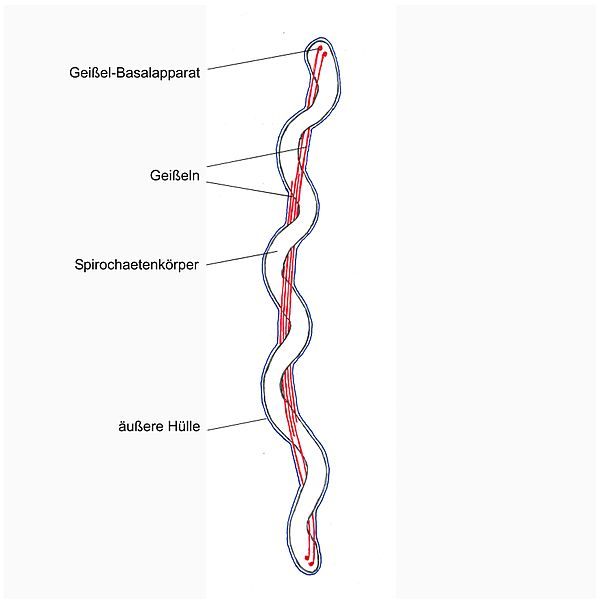
\includegraphics[scale=0.42]{./pictures/schema_spiro_596}
		\end{center}
		\caption{\slshape{Grobes Schema einer Spirochaetenzelle}}
		\label{fig:spiroschema}
		\end{figure}
			
	\item Erläutern Sie den Lebenszyklus der Chlamydien! Warum sind diese Bakterien (\emph{C. trachomatis}) als Krankheitserreger so bedeutsam?
		
		Chlamydien sind obligate intrazelluäre Parasiten.
		Sie reduzieren die Stoffwechselleistung der Zellen und werden deshalb auch als ``Energieparasiten'' bezeichnet.
		Chlamydien können in zwei Formen auftreten.
		Der sogenannten ``Elementary body'' kommt außerhalb von Zellen vor und dringt
		durch Phagocytose in die Wirtzelle ein.
		Nun wandelt er sich zum sogenannten ``Reticulate body'',
		der zweiten Form der Chlamydien,
		und vermehert sich.
		Nach dem genug ``Reticulate bodies'' endstanden sind,
		wandeln sich diese wieder in ``Elementary bodies'' um und verlassen den Wirt um andere Zellen zu besiedeln.

		Chlamydien Infektionen bleiben oft unendekt,
		da sie symptomlos verlaufen.
		So können sich die Bakterien im Uro-Genitaltrakt einnisten
		und Unfruchtbarkeit auslösen.
		Im Auge kann \emph{C. trachomatis} ein Infektion auslösen die zur Erblindung führt.

	\item Die Cyanobakterien sind eine extrem erfolgreiche Bakteriengruppe: Sie leben nicht gerade von Luft und Liebe, aber trotzdem von sehr einfachen Verbindungen. Nennen Sie C-Quelle, N-Quelle, Elektronendonor und Energiequelle dieser Bakterien!
		\begin{description}
			\item[C-Quelle]	\ce{CO2}, Glukose
			\item[N-Quelle]	Nitrate, Ammonium, \ce{N2}-Fixierung
			\item[Elektronendonor] 	Wasser (oxygene Photosynthese)
			\item[Energiequelle]		Licht
		\end{description}

	\item Glauben Sie, dass ein solch vielfältiges Leben, wie wir es auf der Erde kennen, möglich wäre, wenn es die oxygene Photosynthese nicht geben würde?

		Nein. Aber ich sollte das in der Bibel nachlesen.

	\item Cyanobakterien und -Proteobakterien können leicht mit eukaryontischen Zellen interagieren. Nennen Sie ein paar Beispiele für solche Interaktionen (mindestens sechs)!
	
		\begin{itemize}
			\item Plastiden \hfill (Chloroplasten, Rhodoplasten
			\item Symbiosen \hfill (Lebermoose, Cycadeen, Farnen)
			\item Sybiose mit Anabena - Azolla \hfill (N-Quelle für Reis)
			\item phototophe Komponente von Flechten
		\end{itemize}

	\item Was sind die Schritte, einen künstlichen Organismus herrzustellen? Halten Sie das für eine gute Idee?

		\begin{itemize}
			\item Minimales Gensets ermitteln
			\item Assemblierung des künstlichen Minimalgenoms aus Oligonukleotiden
			\item Assemblierung zu Chromosomen
			\item Einführen des künstlichen Genoms in ein Zelle deren DNA zuvor entfernt wurde
		\end{itemize}

	\item Milchsäurebakterien spielen für viele biotechnologische Vorgänge in der Nahrungsmittelindustrie eine große Rolle. Was unterscheidet homo- und heterofermentative Milchsäurebakterien? Sie erhalten die Aufgabe, ein heterofermentatives Bakterium in ein homofermentatives zu verwandeln. Wie gehen Sie vor?

		Bei der homofermentativen Milchsäuregärung wird die Glykolyse anders durchgeführt.
		Da bei heterofermentativen Milchsäure gäreren die Aldolase fehlt,
		verwenden sie den Pentosephosphat-Weg.
		Deshalb endsteht bei ihnen als Endprodukt zusätzlich Ethanol.

	\item Streptomyceten sind wichtige Antibiotikabildner. Nennen Sie einige von Streptomyceten gebildete Antibiotika und die Erreger, die man damit bekämpfen kann. Warum sterben eigentlich die Streptomyceten nicht selbst an den von ihnen gebildeten Antibiotika?

		In Tabelle \ref{tab:strpetoantibiose} befindet sich ein Übersicht über die von Streptomyceten gebildeten Antiobiotika.
		
		\begin{table}[h!]
		\begin{center}
		\begin{tabular}{l l l l} 
		\toprule
		Gruppe			&	Name				&	Produzent			& 	wirksam gegen	\\
		\midrule
		Aminoglcycine	&	Streptomycin	&	S. griseus			&	Gram-negative		\\
		\multirow{2}{*}&	Spectinomycin	&	S. spp.				&	M. tuberculosis		\\
							&	Neomycin			&	S. fradiae			&	Breitband		\\
		Tetracycline	&	Tetracyclin		&	S. aureofaciens	&	Breitband		\\
		Macrolide   	&	Erythromycin	&	S. erythreus		&	meiste Gram-positive		\\
		Polyene     	&	Nystatin			&	S. noursei			&	Pilze		\\
		keine       	&	Chloramphenicol&	S. venezuelae		&	Breitband		\\
		\bottomrule
		\end{tabular}
		\label{tab:strpetoantibiose}
		\caption{Übersicht über die Antibiotika Produczenten der \emph{Streptomyceten}.}
		\end{center}
		\end{table}

		Durch Verschiedene Mechanismen können sich die Strptomyceten vor ihren eigenen Antibiosen schützen.
		Durch Methylierung der eigenen rRNA geht der zum Beispiel der Angriffsort verloren.
		Dies geschieht auch durch veränderung der nicht ribosomalen Ziele,
		wie der DNA-Gyrase, der RNA-Polymerase und EF-Tu. %das gehoert zu tRNA und bindet AS im 50S ribosom o0
		Weiterhin werden die Inhibitoren der Translation durch Phosphorylierung,
		Acetylierung und Glykoylierung modifiziert.

	\item Wofür steht das E. in \emph{E. coli}? 

		Escherichia.
		%bam!

	\item Ralstonia eutropha wurde in Weende entdeckt. Welche Eigenscaften machen dieses Bakterium so interessant?
		
		Das Bakterium ist in der Lage Polyhydroxybuttersäure.
		Diese kann verwendet werden,
		um Biopolymere zu erzeugen.
		Durch Zugabe von bestimmten Stoffe kann man dann Plastik-artige Materialien erzeugen,
		welche jedoch biologisch abbaubar sind.

	\item Zu den Gamma-Proteobakterien gehören die Enterobakterien. Nennen Sie einige Vertreter dieser Bakteriengruppe!
	
		\begin{itemize}
			\item Legionella pneumophila	\hfill (pathogen)
			\item Vibrio cholerae
			\item Photobacterium
			\item Haemophilus influenzae 	\hfill (pathogen)
			\item Acinetobacter calcoaceticus
			\item	Pseudomonas aeruginosa 	\hfill (pathogen)
			\item Azotobacter vinelandii
			\item	Xylella fastidiosa 	\hfill (pathogen)

		\end{itemize}

		Fakultative Anaerober, die alle sehr nahe miteinander verwandt sind.

	\item Zu den Delta-Proteobakterien gehören die Gattungen Myxococcus, Bdellovibrio und Geobacter. Nennen Sie die wichtigsten Eigenschaften bzw. Charakteristika dieser Bakterien!
		
		\begin{description} 
			\item[Myxococcus] \hfill \\
				Sozial-lebende Proteobacterien, die komplizierte Strukturen ausbilden.
				Sie sind beweglich und machen bei reichem Nährstoffangebot einer schwärmende Bewegung.
				Bie Nährstoffarmut erfolgt ein zusammenziehen und das bilden von Fruchtkörpern aus etwa 10.000 Zellen.
				Ernähren sich auch von anderen Bakterien, beispielsweise \emph{E. coli}.
				Die Fruckkörper können bis zum 1 mm  groß werden.
			\item[Bdellovibrio] \hfill \\
				Lebt parasitär an anderen gram-negativen Bakterien.
				Sie lagern sich ein ins Periplasma,
				in dem nun als Bdelloplasten an und saugen den Wirt aus.
			\item[Geobacter] \hfill \\
				Anaerobe Atmung, mit ungewöhnlichen Elektronenakzeptoren (z.B. Uran).
		\end{description}

\end{enumerate}

\newpage
\section{Viren und Prionen}
\begin{enumerate}
	\item Welche subzellulären Krankheitserreger kennen Sie? Bei welchen Organismengruppen können diese Erreger Krankheiten auslösen?
		
		\begin{itemize}
			\item Viren
			\item Viroide
			\item Prionen
			\item Phagen
		\end{itemize}
		
		In allen Domänen des Lebens gibt es spezielle Viren und Phagen.

	\item In welchen Zustandsformen können Viren und Phagen nach der Infektion in der Zelle vorliegen!

		\begin{description}
			\item[Replikationsaktiver Zustand] \hfill \\
				Eine aktive Replikation der Viren findet statt und es werden Nachkommenvieren gebildet.
				%klingt komisch ist aber so.
			\item[Latenzzustand (Lysogenie)] \hfill \\
				Die Zelle ruht mit dem ins Genom integriertem Virus.
		\end{description}

	\item Welches genetische Material besitzt das HI-Virus? 
		
		ss RNA Retroviren - Verletz das zentrale Dogma der Molekularbiologie!\\
		\vspace{1cm}
		reverse Transcriptase(ss RNA) \textrightarrow ds DNA \ldots

	\item Erläutern Sie kurz den Lebenszyklus des Phagen Lambda!

		Die Phage Lambda kann sich nach der Infektion in einen lysogenen Zyklus
		und einen lytischen Zyklus.
		Wobei letzterer für die Vermeherung und weitere Verbreitung dient.
		Im lysogenen Zyklus wird das Genom der Phage in das Genom des Wirtes eingebaut und kann dort überdaueren.
		Durch UV-Strahlung wird der lytische Zyklus ausgelöst.

	\item Bei der spongiformen Enzephalitis kann eine erblich bedingte Krankheit infektiöse Erreger hervorbringen. Wie ist das möglich?
		
		Gerstmann-sträußler-Sheinker / fCJD ist erblich übertragbar,
		aber alle Prionen erzeugen ein Prionenprotein welches infektiös ist.

\end{enumerate}
